\section{The retail graph}

\subsection{Background}
The spend data has been extracted and made available in csv format.The data includes the following headers.  Each row is represents a single transaction.
\subsection{Naming explanation}
\begin{itemize}
  \item \textbf{\_id} A unique identifier from the MongoDB collections.
  \item \textbf{Dedupegroup} A client number, for lookups in the datawarehouse.
  \item \textbf{Seg\_L3\_Num} Level 3 client segmentation number.
   \item \textbf{Seg\_L3\_STR} Level 3 client segmentation dscription.
  \item \textbf{TransactionAmount} The amount of the transaction, negative for money flowing from an account.  Inflows are such as refunds are positive.
  \item \textbf{TransactionDate} Date of transaction format \newline 'yyyy-mm-ddTHH:MM:SS.fffZ'
  \item \textbf{dayname} String description of day, ie Sunday, Monday etc.
  \item \textbf{period} The period of transaction, yyyyMM.
  \item \textbf{month} A client number, for look ups in the data-warehouse.
  \item \textbf{universaldate} A retail short date.  The first Sunday of every month is labelled the 1st, the first Monday of every month is labelled the 2nd etc.
  \item \textbf{weekday} Integer representing the day of the week.
  \item \textbf{weekth} The week of the year number.
  
  \item \textbf{companyindex} A unique identifier for classified companies.
  \item \textbf{companyname} A unique string name for classified companies.
  \item \textbf{franchisename} A unique string name for a merchant.
  
  \item \textbf{class\_id} Class identifier of company.
  \item \textbf{subclass\_id} Sub-class identifier of company.
  \item \textbf{group\_id} Group identifier of company.
  \item \textbf{division\_id} Division identifier of company.
  \item \textbf{discretionary} Classifying the type of spend at a classified company.
  \item \textbf{channel} Transaction mode description.

  \item \textbf{db} Name of source db.
  \item \textbf{dbprefix} Name of source table.
\end{itemize}


\subsubsection{Name convention}
Enforce a standard parameter naming convention.  Where possible we keep the origin names.  Small caps an underscore word separation:

\begin{center}
 \begin{tabular}{||r l||} 
 \hline
 Import & Neo4J  \\ [0.5ex] 
 \hline\hline
 Dedupegroup & dedupestatic \\ 
 Seg\_L3\_Num & seg\_l3\_num \\
 Seg\_L3\_STR & seg\_l3\_str \\
 TransactionAmount & transactionamount \\
 TransactionDate & transactiondate \\
 dayname & dayname \\ 
 period & period \\ 
 month & month \\ 
 
 universaldate & universaldate \\ 
 weekday & weekday \\
 weekth & weekth \\
 companyindex & companyindex \\
 companyname & companyname \\ 
 franchisename & franchisename \\  
 class\_id & class\_id \\ 
 subclass\_id & subclass\_id \\ 
 group\_id & group\_id \\
 division\_id & division\_id \\
 discretionary & discretionary \\ 
 channel & channel \\ 
 db & db \\ 
 dbprefix & dbprefix \\
 \hline
\end{tabular}
\end{center}


The retail graph consists of two nodes, client and merchant. 

In the graph database we enforce uniqueness constraints on the franchise name of the merchant node and the client identifier on the client node. 

All transactions for the period March 2020 was loaded into a Neo4j graph database. For the purpose of this work we only look at one subset of merchant with subclass\_id = 56101.  These are known as the 'fast food' brands or formally 'Food service activities of take away counters', loosely as some offer sitdown services, blurring the line between a restaurant and a entity known traditionally as a fast food restaurant.

\subsubsection{The client node}
The client node has the following properties:
\begin{itemize}
%   \item \textbf{\_id} A unique identifier from the MongoDB collections.
  \item \textbf{dedupestatic}  This is the client identifier and has a uniqueness  constraint placed on it.
  \item \textbf{seg\_l3\_num}
   \item \textbf{seg\_l3\_str}
   \item \textbf{period}   
  \item \textbf{totaltransactionamount} The aggregated value of all transactions performed by this client.
  \item \textbf{totaltransactioncount} The aggregated count of all transactions performed by this client.
%   \item \textbf{transactiondatelist} A list of the dates on which a transaction occurred.
\end{itemize}

 An example of two client nodes and their properties are shown in table \ref{tab:twoclientproperties}.  Some of the properties will be explained later.  Client nodes can contain any number of (client) properties.

\begin{center}
\begin{table}[htb!]
    \centering
    \begin{tabular}{lll}
    \toprule
    %  \hline
                      Attribute &                              client 1 &                                client 2 \\
    %  \hline\hline
    \midrule
                         period &                                202003 &                                  202003 \\
        % triadic\_community &                                  7916 &                                    7916 \\
    %  client\_link\_community\_7916 &                                  1415 & 1415 \\
                     seg\_l3\_num &                                   324 &                                     312 \\
         total transaction amount &                              -5027.83 &                                 -674.93 \\
          total transaction count &                                    30 &                                      10 \\
                %   dedupestatic &                       1.940665861e+11 & 1.919770742e+11 \\
    %  client\_link\_community\_6241 &                                  1421 &                                 1336928 \\
% seg\_l3\_str &  CB - PBCVM - Middle Market - Matured &  CB - PBCVM - Mass Market - Traditional \\
    \bottomrule
    \end{tabular}
    \caption{Two clients and their properties}
    \label{tab:twoclientproperties}
\end{table}
\end{center}

Visually these two nodes appear on screen as figure \ref{fig:twoclientnodes}.

\begin{figure}[ht]
\caption{Two client nodes}
\centering

\includegraphics[width=\textwidth]{png/graph_client12.png}
\label{fig:twoclientnodes}
\end{figure}

\subsubsection{The merchant node}

The merchant node has the following properties:

\begin{itemize}

  \item \textbf{totaltransactionamount} The total amount spent at this merchant by all clients.
  \item \textbf{totaltransactioncount} The total number of transactions by all clients at this merchant.
  \item \textbf{companyindex} This is a number assigned to a company.  A company may have many merchants and many merchant nodes will have the same companyindex.
  \item \textbf{companyname} The name of the company that is the owner of the merchant.  The relationship between company to merchant is therefore one to many.
  \item \textbf{franchisename} This is the name of the node, or the merchant name.  This name provides more detail, such as an implicit reference to the location of the merchant.
%   \item \textbf{period} 
 \item \textbf{class\_id} The class identifier of the company.
  \item \textbf{subclass\_id} Sub-class identifier of company.
  \item \textbf{group\_id} Group identifier of company.
  \item \textbf{division\_id} Division identifier of company.
  \item \textbf{discretionary} Classifying the type of spend at a classified company.  This is a subjective classification.
\end{itemize}

An example of two merchant nodes and their properties are shown in table \ref{tab:twomerchantproperties}.  Merchant nodes can contain any number of (merchant) properties.

\begin{center}
    \begin{table}[htb!]
        \centering
    \begin{tabular}{lll}
    \toprule
        %  \hline
                   attribute &      merchant 1 &  merchant 2 \\
    %  \hline\hline                   
    \midrule
                      period &          202003 &      202003 \\
                 
        %   triadic\_community &            7242 &        7242 \\
     triadic\_56101\_community &            7916 &        7916 \\
                 companyname &             KFC &         KFC \\
                companyindex &              65 &          65 \\   
               discretionary &               2 &           2 \\
                     channel &               0 &           0 \\
                 division\_id &              56 &          56 \\
                    group\_id &             561 &         561 \\   
                    class\_id &            5610 &        5610 \\ 
                 subclass\_id &           56101 &       56101 \\                   
               franchisename &  KFC PHOLA PARK &  KFC MOLOTO \\                 
      totaltransactionamount &         -3509.3 &    -20780.8 \\                 
       totaltransactioncount &              37 &         206 \\
    \bottomrule
    \end{tabular}
        \caption{Two merchants and their properties}
        \label{tab:twomerchantproperties}
    \end{table}
\end{center}


Visually these two merchant nodes appear on screen as figure \ref{fig:twomerchantnodes}.

\begin{figure}[ht]
\caption{Two merchant nodes}
\centering

\includegraphics[width=\textwidth]{png/merchant12.png}
\label{fig:twomerchantnodes}
\end{figure}

% \begin{center}
%     \begin{tabular}{lllll}
% \toprule
%      \hline
%          attribute &   client 1  &  client 1    \\
%               \hline\hline
% \midrule
%             period &        202003 &        202003  \\
%             merchant & KFC PHOLA PARK &  KFC MOLOTO  \\
%  transactionamount &         -54.9 &         -31.9 \\
%         %   dbprefix &        CMProd &        CAProd &        CAProd &        CAProd \\
%   transactioncount &             1 &             1 \\
%                 % db &  CMProd202003 &  CAProd202003 &  CAProd202003 &  CAProd202003 \\
% \bottomrule
% \end{tabular}
% \end{center}


% \begin{center}
%     \begin{tabular}{lllll}
% % \toprule
%      \hline
%          attribute &    client 2  &  client 2  \\
%               \hline\hline
% % \midrule
%             period &           202003 &        202003 \\
%             merchant & KFC PHOLA PARK &  KFC MOLOTO \\
%  transactionamount &          -19.9 &         -49.8 \\
%         %   dbprefix &        CMProd &        CAProd &        CAProd &        CAProd \\
%   transactioncount &             1 &             2 \\
%                 % db &  CMProd202003 &  CAProd202003 &  CAProd202003 &  CAProd202003 \\
% % \bottomrule
% \end{tabular}
% \end{center}


\subsubsection{The transaction relationship}
All transactions between a client and one merchant are represented by a single relationship named TRANSACTED\_AT.  The direction is from client to merchant.  This relationship has the following properties:

\begin{itemize}
  \item \textbf{totaltransactionamount} The total amount of all transactions between a client and a merchant.
  \item \textbf{totaltransactioncount} A running count of the number of transactions between a client and a merchant.  
%   \item \textbf{db} Name of source db for this transaction.
%   \item \textbf{dbprefix} Name of source table for this transaction.
\end{itemize}

An example of how merchant and client nodes are related by means of a transaction, is given in figure \ref{fig:graphexample} on page , for one client and two merchants. 

\begin{figure}[htb]
\caption{Client and Merchant relationship}
\centering
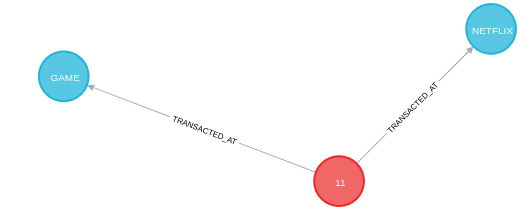
\includegraphics[width=\textwidth]{graphexample.png}
\label{fig:graphexample}
\end{figure}

This client may have visited many more merchants, not shown here in this simple representation, and the merchants shown here in turn in all likelihood were visited by many more clients.

Two clients may also be linked in  a similar manner, by virtue of having transacted at the same merchant. Similarity between clients increase as more merchants are added into the equation.  On a company level, similarity has a preference flavour, while on the level of a merchant, similarity also has a distinct geographical implication.

Extending the above examples, a client may have transacted at two merchants during a month and another client may have done the same, visiting exactly the same merchants, see the example in figure \ref{fig:two clients_two merchants}.

\begin{figure}[htb!]
\caption{Two clients and two merchants}
\centering
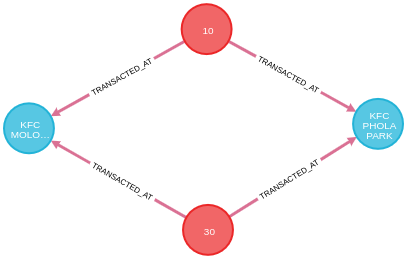
\includegraphics[width=\textwidth]{png/client_merchant_graph.png}
\label{fig:two clients_two merchants}
\end{figure}

\subsubsection{Merchant-merchant relationships}


The Louvain method is one way of detecting communities in large graphs such as the South African (Nedbank) retail network.  The Louvain algorithm is a hierarchical clustering tool.  By employing such clustering we should be able to extract geographical communities of merchants such as found in malls or defined by infrastucture and convenience. The viability of new merchants and credit quality of existing merchant may be enriched by such knowledge.

\subsubsection{Creating client relationships}

\begin{center}
\begin{tabular}{rr}
\toprule
 client count &  client\_link\_community \\
\midrule
    48 &                    822 \\
   108 &                    232 \\
   112 &                     44 \\
   146 &                     86 \\
   172 &                   1415 \\
   206 &                     27 \\
   237 &                    220 \\
   238 &                   1779 \\
   288 &                     95 \\
   333 &                     75 \\
   372 &                     31 \\
   429 &                    176 \\
\bottomrule
\end{tabular}
\end{center}


\subsubsection{The Merchant Edge}

The merchant edge is the link between two merchants when a single client have transacted at both as depicted in fig \ref{fig:graphexample}.  This merchant-merchant relationship, here called TRIADIC\_MERCHANT\_FEET\_LINK, see fig \ref{fig:triadic_closure}, is said to close the triangle between client and two merchants. 
Clients make a choice to visit and transact at more than one merchant. The period under consideration may be extended to include all history for a client in which case the preference and geographical insight will presumably be much weaker.  At the other extreme the period may be restricted to a particular day.  In such an event, triadic closure is only achieved when a transaction is concluded at two merchants on the same day.  

\begin{figure}[htb!]
\caption{Triadic closure between merchants}
\centering
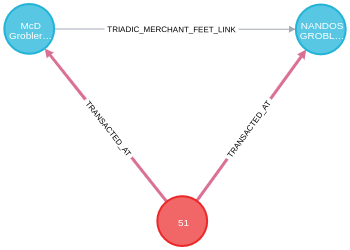
\includegraphics[width=\textwidth]{triadic_closure.png}
\label{fig:triadic_closure}
\end{figure}

TRIADIC\_MERCHANT\_FEET\_LINK has three properties.  All three properties are the result of a transaction count, as opposed to transaction value, and hence the reference to feet.  Given a merchant A and a merchant B, the first is \textbf{count}, which is the number of clients who transacted at both merchants A and B, count also provides a means of attaching a weight to TRIADIC\_MERCHANT\_FEET\_LINK and a convenient means of eliminating weak and spurious relationships.
The second property is a count of all transactions performed at A by clients who transacted at A and B, ID0.  The third property is similarly the count of all transactions performed at B by clients who transacted at A and B, ID1.  ID0 and ID1 provides a means of establishing a direction for the merchant feet edge: if ID0\<ID1, then the merchant edge points in the direction of B and in the direction of A if ID1\<ID0.  The direction property of TRIADIC\_MERCHANT\_FEET\_LINK becomes important when ranking merchants.
These three properties provide the strength of the edge between A and B but also a means to attach a direction to the edge by pointing it in the direction of the net count of transactions.
Triadic closure creates a relationship between two merchants that were not immediately apparent from the data.

\paragraph{The value edge}

The value edge also establishes a direction of a merchant edge.  Using a transaction value for each of the linked merchants, but only for clients who shopped at merchant A and also B, if the total value of all transactions for this client at B is larger than at A the 'value' for this client is flows from A to B for this client.  When aggregated over the period for all clients an aggregated 'value' direction is established.

\subsection{Merchant communities}

The Louvain method is one way of detecting communities in large networks.  The Louvain algorithm is a hierarchical clustering tool.  By employing such clustering we should be able to extract geographical communities of merchants such as found in malls or defined by other infrastucture. The viability of new merchants and credit quality of existing merchant may be enriched by such knowledge.

We limit ourselves to fast food restaurants or subclass\_id = 56101.

In table \ref{tab:sa_fastfood_communites} are the most dominant communites of Sout african fastfood merchants.  Community 7916 has the least number of fast food merchant being 25. 

\begin{center}
    \begin{table}[]
        \centering
            \begin{tabular}{rr}
            \toprule
             Number of merchants &  SA Fast food community by ID \\
            \midrule
                      25 &                     7916 \\
                      30 &                     2697 \\
                      32 &                     6246 \\
                      44 &                     6305 \\
                      55 &                     6314 \\
                      61 &                      290 \\
                      69 &                     6790 \\
                      72 &                     8577 \\
                      84 &                     2160 \\
                      96 &                     5959 \\
                     109 &                     6244 \\
                     115 &                     7805 \\
                     122 &                     7579 \\
                     128 &                     1875 \\
                     149 &                     7544 \\
                     187 &                     5898 \\
                     241 &                     4914 \\
                     258 &                      154 \\
                     319 &                     6778 \\
                     351 &                     5936 \\
                     364 &                     6365 \\
                     398 &                     8188 \\
                     517 &                     1772 \\
                     765 &                     5989 \\
            \bottomrule
            \end{tabular}
        \caption{South African fast food communities}
        \label{tab:sa_fastfood_communites}
    \end{table}
\end{center}

Some fast food merchant do not belong to any communities as not all merchants fulfil the requirements which may for a variety of reasons.
Having defined these communities one can now ask which of the (merchant) node is the most influential, a question similar the answer provided by the Google page rank algorithm (see reference).  The relevance of the 'merchant' rank could be manifold.  The highest ranked merchant could be subject to the most severe competition, but could also be seen to be at the center of a particular market and in the most lucrative area.  The merchant rank for fast food community 7916  is given in \ref{tab:merchant_community_7916}.  KFC Groblersdal is determined to be at the (transactional) heart of this cluster, based on its merchant rank.

\begin{center}
    \begin{table}[]
        \centering
            \begin{tabular}{lr}
            \toprule
               franchisename &     score \\
            \midrule
                KFC GROBLERS &  0.809422 \\
              NANDOS GROBLER &  0.670787 \\
                DEBONAIRS SI &  0.660889 \\
                KFC MOUTSIYA &  0.601046 \\
              WIMPY GROBLERS &  0.575624 \\
                KFC KWAGGAFO &  0.470889 \\
              STEERS MORATIW &  0.441075 \\
              DEBONAIRS GROB &  0.394640 \\
                  KFC MOLOTO &  0.277500 \\
                McD Kwagga M &  0.267938 \\
                McD Groblers &  0.259299 \\
                KFC MOUTSE M &  0.232283 \\
              KFC MOUTSIYA M &  0.213750 \\
                KFC PHOLA PA &  0.195549 \\
              DEBONAIRS MORA &  0.186734 \\
              DEBONAIRS SIYA &  0.186734 \\
              DEBONAIRS JANE &  0.150000 \\
              KFC GROBLERSDA &  0.150000 \\
                KFC JANE FUR &  0.150000 \\
                KFC MARBLE H &  0.150000 \\
                KFC Moratiwa &  0.150000 \\
              KFC PHOLA PARK &  0.150000 \\
                KFC SIYABUSW &  0.150000 \\
               KFC SIYABUSWA &  0.150000 \\
             McD Groblersdal &  0.150000 \\
            \bottomrule
            \end{tabular}
        \caption{Most prominent merchants in community 7916}
        \label{tab:merchant_community_7916}
    \end{table}
\end{center}

By repeating the merchant rank algorithm for each cluster we find the centers of all merchant (fast food) clusters.  In table \ref{tab:summary_fastfood_clusters} is listed the centers of all fast food merchant clusters, their geographical name (loosely based on the closest town) the number of merchants ffound in the cluster and the name of the cluster as it is found in the database as well as the community number.  The latter is a arbitrarily chosen number from the algorithm.


\begin{center}
    \begin{table}[htb]
        \centering
            \begin{tabular}{rlrl}
            \toprule
             community &              area &  membercount & franchisename\_1 \\
            \midrule
                7916.0 &       Groblersdal &           25 &    KFC GROBLERS \\
                2697.0 &         Bethlehem &           30 &  MCD Phuthaditj \\
                6246.0 &       Ventersdorp &           32 &    STEERS VENTE \\
                6305.0 &         Worcester &           44 &  STEERS RESTAUR \\
                6314.0 &        Klerksdorp &           55 &    WIMPY GOUDKO \\
                 290.0 &       Port Edward &           61 &  KFC IZINGOLWEN \\
                6790.0 &         Kimberley &           69 &    KAUAI KIMBER \\
                8577.0 &    Vanderbijlpark &           72 &    MCDONALD'S V \\
                2160.0 &        Emalahleni &           84 &  WIESENHOF COSM \\
                5959.0 &         Nelspruit &           96 &    KFC NELSPRUI \\
                6244.0 &      Bloemfontein &          109 &    STEERS PRELL \\
                7805.0 &  Pietermaritzburg &          115 &    MCDONALD'S C \\
                7579.0 &        Rustenburg &          122 &    KFC SUN VILL \\
                1875.0 &           Makhado &          128 &    NANDOS MAKHA \\
                7544.0 &            Eshowe &          149 &    NANDOS ESHOW \\
                5898.0 &    Port Elizabeth &          187 &    WIMPY METLIF \\
                4914.0 &       East London &          241 &    KEI STEERS D \\
                 154.0 &         Centurion &          258 &  BURGER KING JE \\
                6778.0 &        Wonderboom &          319 &  MCD Sammy Mark \\
                5936.0 &          Alberton &          351 &    WIMPY NEW RE \\
                6365.0 &      Kempton Park &          364 &    SPUR BRAVE H \\
                8188.0 &           Florida &          398 &    WIMPY FLORID \\
                1772.0 &         Umhlangha &          517 &  MCD MountEdgec \\
                5989.0 &         Cape Town &          765 &   MCD Vangate ( \\
            \bottomrule
            \end{tabular}
            \caption{Summary of SA fast food clusters}
        \label{tab:summary_fastfood_clusters}
    \end{table}
\end{center}

There is therefore 24 easily discernible fast food merchant clusters for March 2020.
\subsection{Merchant communities}

\subsection{The Merchant Rank}

Two graphs exist each sharing the Merchant nodes.  One has Merchants connected via the MERCHANT\_FEET\_LINK and the other via the MERCHANT\_FEET\_LINK

\subsubsection{The Client Edge}

